
\section{Úvod}
%Zajištění bezpečnosti jaderného zařízení, resp. jaderného reaktoru je primárním cílem od výstavby, provozu až po vyřazení z provozu. Jedním z mnoha prostředků sloužících k zajištění bezpečnosti jaderného zařízení jsou bezpečnostní analýzy, které se dělí na deterministické analýzy (neutronické, termohydraulické, termomechanické, strukturální a radiační) a pravděpodobnostní hodnocení zařízení. K deterministickému hodnocení bezpečnosti jsou třeba kvalifikované nástroje, čímž jsou mimo jiné také systémové termohydraulické kódy (SYS-TH - system thermal hydraulics). \cite{bestion2017structure, SUJB_zprava}
Systémové termohydraulické kódy (SYS-TH) tvoří nedílnou součást bezpečnostních analýz. Simulace poskytují informace o příslušných parametrech systému, jako jsou tlak, teplota chladiva nebo průtok v kontrolních objemech a teploty materiálů v modelovaných strukturách, to vše v závislosti na čase. SYS TH kódy jsou obvykle založeny na řešení pěti nebo šesti nehomogenních rovnic zachování hmotnosti, energie a hybnosti, obvykle s použitím implicitních nebo poloimplicitních schémat. Prostřednictvím těchto kódů lze simulovat provoz a chování reaktoru, včetně průběhu havárií, a posoudit tak úroveň bezpečnosti jaderné elektrárny \cite{bestion2017structure, petruzzi2008thermal}.

\section{Oblasti aplikace}
Systémové kódy jsou považovány za multifyzikální výpočetní programy schopné simulovat jak základní fyzikální jevy (např. var na stěně trubky), tak i celistvé chování systémů (např. primárního okruhu jaderné elektrárny). Díky tomu je možné pomocí těchto kódů počítat i složité přechodové jevy, které mohou představovat například základní projektové události a nehody na jaderném zařízení. Kromě termohydraulického popisu přenosu hmoty, hybnosti a energie je možné aplikovat SYS-TH kódy na:
\begin{itemize}
	\item popis transportu plynů ($ \text{N}_{2},\,\text{H}_{2},$ vzduch, produkty štěpení...),
	\item transport bórů a těkavých plynů,
	\item kondukce skrze materiály s konvekcí do tekutin,
	\item zjednodušený neutronický popis,
	\item chemický popis reakcí zinku s vodou,
	\item popis chování paliva,
	\item popis chování součástek jaderných elektráren jako rotorů či ventilů,
	\item popis řídících systémů (Instrumentation \& Control).
	
\end{itemize}

V oblasti jaderného inženýrství se používá řada nejmodernějších termohydraulických kódů. Mezi nejpoužívanější kódy patří RELAP5, TRACE, APROS, POLKA-T, CATHARE, ATHLET a RETRAN. Tyto kódy využívají přístup založený na kontrolních objemech s velkou nodalizací a aplikují nejmodernější termohydraulické modely k popisu fyzikálního chování systému \cite{petruzzi2008thermal}.
\section{Hodnocení systémových kódů}
Nedílnou součástí vývoje numerických SYS-TH kódů a jejich interního hodnocení je verifikace a validace. Verifikace i validace se týká procesu zvyšování spolehlivosti kódu a snižování rizika nesprávné aplikace. Interní hodnocení kódu obvykle provádí vývojář kódu.


Verifikace kódu se týká zkoumání zdrojového kódu ve vztahu k jeho popisu v dokumentaci. Tento proces zahrnuje postupy související se zajištěním kvality softwaru a úsilí o odhalení a opravu chyb v modelech a numerických algoritmech využívaných k řešení parciálních diferenciálních rovnic \cite{petruzzi2008thermal}.

Validace kódu zahrnuje vyhodnocení přesnosti předpovídaných hodnot porovnáním s příslušnými experimentálními údaji. Validace kódu se v podstatě zaměřuje na kvantitativní posouzení přesnosti kódu porovnáním s kvalitními validačními experimenty a benchmarkovými úlohami. Tyto experimenty jsou důkladně zdokumentovány a charakterizovány, včetně pečlivých odhadů statistické chyby měření. Díky validačnímu procesu jsou výsledky kódu konzistentní a prokazují, že celý systém může přinášet smysluplné a očekávané výsledky \cite{petruzzi2008thermal}. Proces interního hodnocení kódu je ilustrován na obrázku \ref{fig:v_v_sean_prezentace}.
\begin{figure}[H]
	\centering
	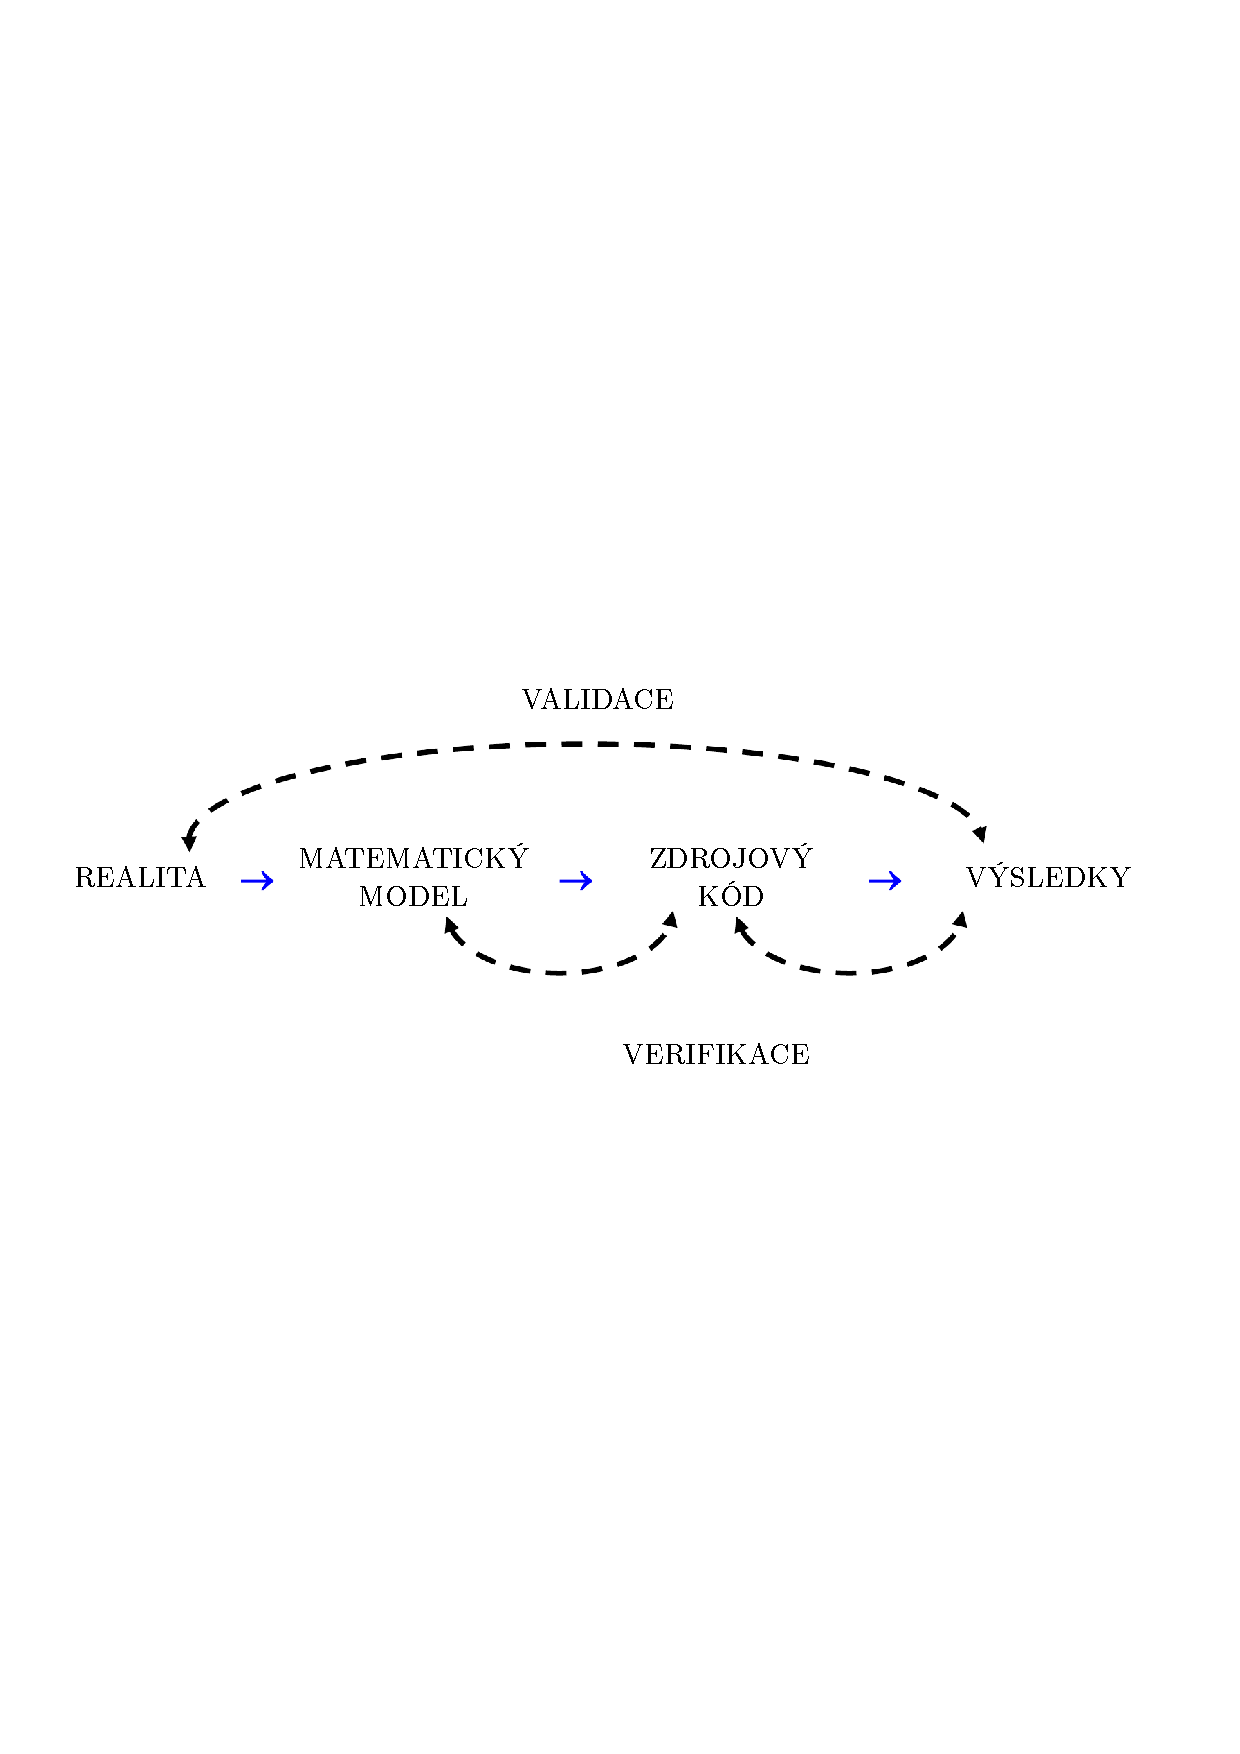
\includegraphics[width=0.8\textwidth, trim={0cm 10cm 0cm 10cm}, clip]{./02_teorie/obrazky/v_v_sean_lectures.pdf}
	\caption{Proces interního hodnocení kódu.}
	\label{fig:v_v_sean_prezentace}
\end{figure}

Interní hodnocení kódu ovšem nemusí vždy identifikovat nepřesnosti kódu při popisu různých fyzikálních jevů. Součástí neustálého vývoje je také externí hodnocení nezávislými institucemi a uživateli. Nezávislé posouzení kódu je proces, kdy třetí strana kvantifikuje přesnost kódu na základě experimentů provedených v integrálním zkušebním zařízení (ITF). Externí posouzení kódu obvykle vyžaduje kvalifikaci uživatele a vhodně zvolenou nodalizaci kontrolních objemů \cite{petruzzi2008thermal}. 

%
%  která je prováděna například srovnáním výsledků s škálovanými experimenty či s daty přímo z jaderné elektrárny. Přestože termohydraulické kódy byly (a stále jsou) za poslední tři dekády neustále vyvíjeny, získávané výsledky jsou stále zatíženy chybami, které mohou být způsobeny nepřesnostmi numerického řešení, nevhodně zvolenými vztahy, nedostatkem znalostí okrajových a počátečních podmínek či efekty nodalizace. 
%\cite{petruzzi2008thermal}


%V závislosti na typu popisované součástky jsou systémové kódy schopné modelovat 0-D, 1-D či 2-D a 3-D geometrie. 0-D model se ve většině případů používá při popisu součástek, ve kterých dochází k velmi nízkým rychlostem proudění, např. kompenzátor objemu. 1-D popis se aplikuje především na součástky s jedním směrem proudění (např. trubky). 2-D a 3-D slouží k analýze součástek náročných na popis (např. AZ reaktoru) \cite{bestion2017structure}. 


\section{Limitace systémových kódů}
Většina užívaných systémových kódů má možnost volné nodalizace jednotlivých termohydraulických komponent. K popisu komplexních problémů se využívají definované komponenty, které jsou děleny na jednotlivé kontrolní objemy. Toto dělení je čistě na uživateli, a neexistuje tedy správný postup, jakou nodalizaci komponent a strukturu studované problematiky použít \cite{petruzzi2008thermal}.

Problematická se může jevit především výše zmíněná nodalizace. Využitím jemnějšího rozdělení je sice možné docílit podrobnějšího popisu, ovšem při nevhodně zvolené nodalizaci, např. přílíš malých kontrolních objemech může docházet k nestabilnímu výpočtu a fyzikálně neodpovídajícím výsledkům. Důvody proč příliš jemná nodalizace může být problematická jsou dva \cite{petruzzi2008thermal}:
\begin{itemize}
	\item velká část empirických vztahů zahrnutých do programu je získána z výpočtu s pevně danou nodalizací, což již z principu vede k rozdílným podmínkám,
	\item numerické simulace využívané v systémových kódech využívají uměle vloženou viskozitu za účelem získání stabilních výsledků.
\end{itemize}

%Dalším aspektem při popisu komplexního problému je propojení jednotlivých součástek, které může mít značný vliv na výsledné proudění. Systémové kódy ve většině případů nabízejí model vytvořit z jednoduchých komponent, a proto je nutné při tvorbě modelu použít "inženýrský odhad" a využít zkušenosti uživatele \cite{petruzzi2008thermal}. 

Důležitá je také široká škála parametrů používaných k popisu fyzikálních jevů. Ne zřídka má uživatel možnost volit mezi dvěma a více vstupními parametry, které k popisu dané problematiky slouží. Příkladem může být například volba mezi různými modely škrcení, nucené proudění podchlazené či nasycené kapaliny nebo nastavení ztrátového součinitele v případě trubek či pístů. Při tvorbě komplexního modelu není neobvyklé, že počet vstupních parametrů se pohybuje v řádu tisíců. Z tohoto důvodu je pravděpodobnost lidské chyby vysoce pravděpodobná a je třeba dbát nesmírné pozornosti při konstrukci modelu. Je vhodné také zmínit často diskutované téma volby časového kroku na řešení a způsobu zadávání okrajových podmínek \cite{petruzzi2008thermal}.

\section{Aplikace na výzkumné reaktory}
Výpočetní kód RELAP5 byl vyvinut jakožto systémový "best-estimate" kód pro popis PIE (postulovaných iniciačních událostí) na konvenčních lehkovodních reaktorech. Množství experimentálně určených vztahů a korelací použitých při vývoji kódu RELAP5 bylo odvozeno a stanoveno právě pro využití na energetických reaktorech, avšak cílem mnohých studií (např. \cite{REIS2012300, CHATZIDAKIS2013341, AZZOUNE2010823}) je aplikace i na výzkumné reaktory \cite{HEDAYAT2017953}. Přestože jsou SYS-TH hojně používány pro bezpečnostní analýzy výzkumných reaktorů, mnohé práce (\cite{international1992iaea, OMAR2010572, CHATZIDAKIS_ASSESMENT_RSG}) upozorňují na nedostatečnou validaci a verifikaci modelů u přechodových jevů a postulovaných iniciačních událostí.  Pro většinu výzkumných reaktorů je kromě jiného také důležitý správný popis odvodu tepla dlouhodobou přirozenou konvekcí. Proto je často kladen důraz na zkušenost uživatele a na \uv{inženýrský odhad} při konstrukci a volbě vstupních parametrů \cite{bestion2017structure}. Z těchto důvodů jsou tvořeny benchmarkové úlohy prováděné právě na výzkumných reaktorech viz např. \cite{international2022iaea_benchmark_database}.

Problém modelování přirozeného proudění se může stát ještě složitějším kvůli přítomnosti dodatečných obtoků a velké redistribuci toku během přechodových jevů. Je na uživateli kódu, aby určil, jak konstruovat takto komplexní proudění v rámci jednorozměrného kódu. K dostatečnému popisu můžou být použity kontrolní objemy, jednoduché a vícenásobné spojovací jednotky či další termohydraulické komponenty. Volba nodalizace a způsobu konstrukce reaktoru by v ideálním případě založena na výsledcích detailních citlivostních analýz. Nicméně v mnoha případech je uživatel nucen učinit ad hoc rozhodnutí kvůli nedostatku času nebo vhodných experimentálních dat \cite{petruzzi2008thermal}.




